\documentclass[11pt]{article}
\usepackage[hmargin=1in,vmargin=1in]{geometry}
\usepackage[table]{xcolor} 
\usepackage{amsmath,amssymb,amsfonts,url,sectsty,tcolorbox,framed}
\usepackage{hyperref}
\usepackage{listings}
\usepackage{booktabs}
\usepackage{array}
\usepackage{multirow}
\usepackage{graphicx}
\usepackage{tikz}
\usetikzlibrary{arrows.meta, positioning, shapes.geometric, fit, backgrounds, calc}
\usepackage{pgfplots}
\pgfplotsset{compat=1.18}
\usepackage{fancyhdr}
\usepackage{fontawesome5}
\usepackage{enumitem}

% ──────────────────────────────────────────────────────
% COLOR PALETTE
% ──────────────────────────────────────────────────────
\definecolor{lightblue}{rgb}{0.8,0.9,1}
\definecolor{codebg}{RGB}{250, 250, 250}
\definecolor{codeframe}{RGB}{200, 200, 200}
\definecolor{tableheader}{RGB}{41, 128, 185}
\definecolor{rowalt}{RGB}{235, 245, 251}
\definecolor{accentblue}{RGB}{52, 152, 219}
\definecolor{accentgreen}{RGB}{39, 174, 96}
\definecolor{accentorange}{RGB}{230, 126, 34}
\definecolor{accentred}{RGB}{231, 76, 60}
\definecolor{accentpurple}{RGB}{142, 68, 173}
\definecolor{darkbg}{RGB}{30, 30, 30}
\definecolor{codekw}{RGB}{86, 156, 214}
\definecolor{codecomment}{RGB}{106, 153, 85}
\definecolor{codestring}{RGB}{206, 145, 120}
\definecolor{codenumber}{RGB}{181, 206, 168}
\definecolor{codetype}{RGB}{78, 201, 176}
\definecolor{sectioncolor}{RGB}{41, 128, 185}

% ──────────────────────────────────────────────────────
% SECTION STYLING
% ──────────────────────────────────────────────────────
\sectionfont{\color{sectioncolor}}
\subsectionfont{\color{sectioncolor!80!black}}
\subsubsectionfont{\color{sectioncolor!60!black}}

% ──────────────────────────────────────────────────────
% HYPERLINK STYLING
% ──────────────────────────────────────────────────────
\hypersetup{
    colorlinks=true,
    linkcolor=sectioncolor,
    urlcolor=accentblue,
    citecolor=accentgreen,
    pdfborder={0 0 0}
}

% ──────────────────────────────────────────────────────
% HEADER / FOOTER
% ──────────────────────────────────────────────────────
\pagestyle{fancy}
\fancyhf{}
\fancyhead[L]{\small\color{gray}\textsc{Lab 7: MPI Point-to-Point}}
\fancyhead[R]{\small\color{gray}\textsc{CS302 -- DPC}}
\fancyfoot[C]{\small\color{gray}\thepage}
\renewcommand{\headrulewidth}{0.4pt}
\renewcommand{\footrulewidth}{0pt}
\fancypagestyle{plain}{\fancyhf{}\fancyfoot[C]{\small\color{gray}\thepage}\renewcommand{\headrulewidth}{0pt}}

% ──────────────────────────────────────────────────────
% CODE STYLE CONFIGURATION 
% ──────────────────────────────────────────────────────
\lstset{
    backgroundcolor=\color{darkbg},
    basicstyle=\ttfamily\small\color{white},
    breaklines=true,
    breakatwhitespace=false,
    commentstyle=\color{codecomment}\itshape,
    keywordstyle=\color{codekw}\bfseries,
    stringstyle=\color{codestring},
    numberstyle=\tiny\color{gray},
    numbers=left,
    numbersep=8pt,
    stepnumber=1,
    frame=none,
    showstringspaces=false,
    language=C++,
    tabsize=4,
    columns=fullflexible,
    keepspaces=true,
    xleftmargin=10pt,
    morekeywords={MPI_Init, MPI_Comm_rank, MPI_Comm_size, MPI_Send, MPI_Recv, MPI_Finalize, MPI_Wtime, MPI_COMM_WORLD, MPI_LONG_LONG, MPI_STATUS_IGNORE},
    emphstyle={\color{codetype}},
    emph={int, bool, long, double, void, const},
    literate=
        {0}{{\textcolor{codenumber}{0}}}1
        {1}{{\textcolor{codenumber}{1}}}1
        {2}{{\textcolor{codenumber}{2}}}1
        {3}{{\textcolor{codenumber}{3}}}1
        {4}{{\textcolor{codenumber}{4}}}1
        {5}{{\textcolor{codenumber}{5}}}1
        {6}{{\textcolor{codenumber}{6}}}1
        {7}{{\textcolor{codenumber}{7}}}1
        {8}{{\textcolor{codenumber}{8}}}1
        {9}{{\textcolor{codenumber}{9}}}1
}

% ──────────────────────────────────────────────────────
% BOX DEFINITIONS
% ──────────────────────────────────────────────────────
\tcbuselibrary{breakable, skins, listings}

\newtcolorbox{codebox}[1][]{%
    enhanced, breakable, colback=darkbg, colframe=darkbg!60!black,
    title={\faCode\ \ #1}, fonttitle=\bfseries\sffamily\small\color{white},
    coltitle=white, arc=4pt, boxrule=0.8pt, top=2pt, bottom=2pt, left=0pt, right=4pt,
    before skip=10pt, after skip=10pt, shadow={1mm}{-1mm}{0mm}{black!30},
    attach boxed title to top left={xshift=10pt, yshift=-\tcboxedtitleheight/2},
    boxed title style={colback=accentblue, arc=3pt, boxrule=0pt, left=6pt, right=6pt}
}

\newtcolorbox{shadedbox}[1][]{%
    enhanced, breakable, colback=lightblue!15, colframe=accentblue,
    title={\faLightbulb[regular]\ \ #1}, fonttitle=\bfseries\sffamily,
    coltitle=white, arc=4pt, boxrule=0.8pt, before skip=10pt, after skip=10pt,
    shadow={1mm}{-1mm}{0mm}{accentblue!20},
    attach boxed title to top left={xshift=10pt, yshift=-\tcboxedtitleheight/2},
    boxed title style={colback=accentblue, arc=3pt, boxrule=0pt, left=6pt, right=6pt}
}

\newtcolorbox{terminalbox}[1]{%
    enhanced, breakable, colback=darkbg, colframe=darkbg!40!black, colupper=white,
    title={\faTerminal\ \ #1}, fonttitle=\bfseries\ttfamily\small\color{white},
    coltitle=white, arc=4pt, boxrule=0.8pt, before skip=10pt, after skip=10pt,
    shadow={1mm}{-1mm}{0mm}{black!30},
    attach boxed title to top left={xshift=10pt, yshift=-\tcboxedtitleheight/2},
    boxed title style={colback=accentgreen!80!black, arc=3pt, boxrule=0pt, left=6pt, right=6pt}
}

\lstdefinestyle{terminalstyle}{
    basicstyle=\ttfamily\small\color{white}, breaklines=true, language=bash, numbers=none,
    literate={>}{{\textcolor{accentgreen}{>}}}1 {-}{{\textcolor{white}{-}}}1,
    columns=fullflexible, keepspaces=true, frame=none, backgroundcolor=\color{darkbg}, xleftmargin=8pt
}

\begin{document}

% ══════════════════════════════════════════════════════
% TITLE PAGE
% ══════════════════════════════════════════════════════
\thispagestyle{empty}
\begin{center}
\vspace*{1cm}

{\color{sectioncolor}\rule{\textwidth}{2pt}}
\vspace{0.3cm}

{\Huge\bfseries\sffamily\color{sectioncolor} Cooperative Computing using MPI}

\vspace{0.15cm}
{\Large\sffamily\color{gray} Point-to-Point Communication: Cracking the Staff WiFi}

\vspace{0.3cm}
{\color{sectioncolor}\rule{\textwidth}{2pt}}

\vspace{1.2cm}

{\large\sffamily\color{sectioncolor} [CS302] Distributed and Parallel Computing}

\vspace{1.5cm}

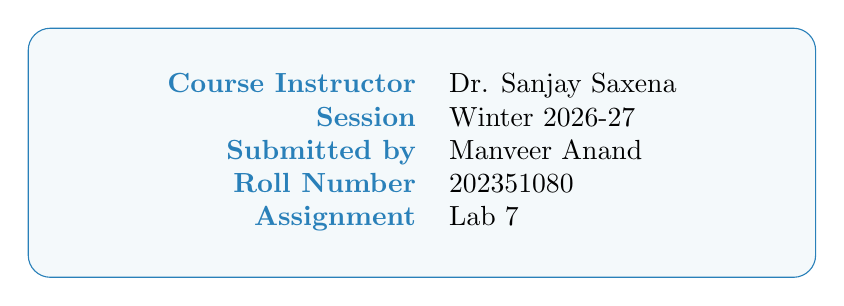
\begin{tikzpicture}
\node[draw=sectioncolor, fill=sectioncolor!5, rounded corners=8pt, inner sep=15pt, minimum width=10cm] {
    \begin{tabular}{r @{\hspace{12pt}} l}
    \textbf{\color{sectioncolor}Course Instructor} & Dr. Sanjay Saxena \\
    \textbf{\color{sectioncolor}Session} & Winter 2026-27 \\
    \textbf{\color{sectioncolor}Submitted by} & Manveer Anand \\
    \textbf{\color{sectioncolor}Roll Number} & 202351080 \\
    \textbf{\color{sectioncolor}Assignment} & Lab 7 \\
    \end{tabular}
};
\end{tikzpicture}

\vspace{1.5cm}

{\color{gray}\small MPI Concepts: \texttt{MPI\_Send} $\cdot$ \texttt{MPI\_Recv} $\cdot$ \texttt{Rank distribution} $\cdot$ \texttt{Point-to-Point}}

\vfill
{\color{gray}\small\today}
\end{center}
\newpage

\tableofcontents
\newpage

% ══════════════════════════════════════════════════════
% INTRODUCTION
% ══════════════════════════════════════════════════════
\section{Introduction}

The objective of this assignment is to model a real-world scenario of cooperative computing between two distributed processes using the Message Passing Interface (MPI). The problem involves two students working together to derive the college staff WiFi password. Since computing the required cryptographic derivations is heavily expensive, the workload is split between two computing nodes (Process 0 and Process 1).

\subsection{Problem Statement}
Two students with roll numbers ending in \textbf{A} and \textbf{B} collaborate. We must simulate a heavy workload using a \textit{Grinder Function} that takes specific seeds and multipliers and iterates two billion times. The overall cooperative flow requires that:
\begin{enumerate}
    \item \textbf{Student 1 (Rank 0)} processes their credentials to compute an $\alpha$ value and sends it to Student 2.
    \item \textbf{Student 2 (Rank 1)} receives $\alpha$, applies a separate heavy derivation to compute a $\beta$ value, and sends it back to Student 1.
    \item Both students compute a common \textit{verification code} to ensure data integrity.
    \item Student 1 leverages both $\alpha$ and $\beta$ to reveal the 4-digit \textit{staff WiFi password}.
\end{enumerate}

\begin{shadedbox}[The Grinder Function]
To simulate a massive cryptographic workload, the \textit{grinder function} executes the following pseudo-random formula \(2 \times 10^9\) times:
\begin{equation}
    r_{next} = (r \times m + a) \pmod{mod\_val}
\end{equation}
where $m$, $a$, and $mod\_val$ are pre-defined constants that vary per computing phase.
\end{shadedbox}

% ══════════════════════════════════════════════════════
% IMPLEMENTATION DETAILS
% ══════════════════════════════════════════════════════
\section{Implementation Details}

This solution was developed using C++ and MPI. Point-to-point communication was strictly enforced using \texttt{MPI\_Send} and \texttt{MPI\_Recv}. 

\subsection{Rank Workflow}
\begin{itemize}
    \item \textbf{Process 0 (Student 1):} Starts execution, calculates $\alpha' = \text{grinder}(A, 31, 17, 9973)$ and $\alpha'' = \text{grinder}(\alpha', 37, 11, 9973)$, sets $\alpha = (\alpha' + \alpha'') \pmod{9973}$, and transmits $\alpha$ via \texttt{MPI\_Send}. It then blocks until $\beta$ is returned.
    \item \textbf{Process 1 (Student 2):} Blocks on \texttt{MPI\_Recv} waiting for $\alpha$. Once received, calculates $\beta'$ and $\beta''$ continuously via the grinder using $B$. Determines $\beta$, transmits it back to Rank 0, and proceeds to verify.
\end{itemize}

\subsection{C++ Source Code (\texttt{staff\_wifi.cpp})}
\begin{codebox}[staff\_wifi.cpp]
\begin{lstlisting}
#include <iostream>
#include <mpi.h>

using namespace std;

// The Grinder Function
// Runs 2 billion times to simulate a heavy workload
long long grinder(long long seed, long long m, long long a, long long mod_val) {
    long long r = seed;
    for (long long i = 0; i < 2000000000LL; ++i) {
        r = (r * m + a) % mod_val;
    }
    return r;
}

int main(int argc, char** argv) {
    MPI_Init(&argc, &argv);

    int rank;
    MPI_Comm_rank(MPI_COMM_WORLD, &rank);

    double start_time = MPI_Wtime();

    long long A = 1080; // Student 1 (202351080)
    long long B = 1114; // Student 2 
    long long alpha, beta, verify;

    if (rank == 0) {
        long long alpha_prime = grinder(A, 31, 17, 9973);
        long long alpha_double_prime = grinder(alpha_prime, 37, 11, 9973);
        alpha = (alpha_prime + alpha_double_prime) % 9973;

        MPI_Send(&alpha, 1, MPI_LONG_LONG, 1, 0, MPI_COMM_WORLD);
        MPI_Recv(&beta, 1, MPI_LONG_LONG, 1, 0, MPI_COMM_WORLD, MPI_STATUS_IGNORE);

        verify = grinder(alpha + beta, 7, 3, 101);
        long long R = grinder(alpha * beta + A + B, 13, 7, 9973);
        long long password = R % 10000;

        double end_time = MPI_Wtime();

        cout << "[Student 1] Verification Code: " << verify << endl;
        cout << "[Student 1] The Staff WiFi Password is: " << password << endl;
        cout << "Total Execution Time: " << (end_time - start_time) << " seconds" << endl;
    } 
    else if (rank == 1) {
        MPI_Recv(&alpha, 1, MPI_LONG_LONG, 0, 0, MPI_COMM_WORLD, MPI_STATUS_IGNORE);

        long long beta_prime = grinder(alpha, B, 13, 9973);
        long long beta_double_prime = grinder(beta_prime, 41, 19, 9973);
        beta = (beta_prime + beta_double_prime) % 9973;

        MPI_Send(&beta, 1, MPI_LONG_LONG, 0, 0, MPI_COMM_WORLD);
        verify = grinder(alpha + beta, 7, 3, 101);

        cout << "[Student 2] Verification Code: " << verify << endl;
    }

    MPI_Finalize();
    return 0;
}
\end{lstlisting}
\end{codebox}

% ══════════════════════════════════════════════════════
% EXECUTION AND RESULTS
% ══════════════════════════════════════════════════════
\section{Execution and Results}

The program was executed on 2 distributed processes using \texttt{mpiexec}. The time metric confirms the computational intensity of performing roughly $6 \times 10^9$ modulo arithmetic operations locally on each node simultaneously. 

\begin{terminalbox}{Terminal Execution Output}
\begin{lstlisting}[style=terminalstyle]
(base) PS D:\Dev 2.0\DPC\LAB 7> .\run_mpi.ps1 "Assignment\staff_wifi.cpp" 2
--> Compiling C++ file Assignment\staff_wifi.cpp...
--> Build successful! Executing with 2 processes...

[Student 2] Verification Code: 22
[Student 1] Verification Code: 22
[Student 1] The Staff WiFi Password is: 4547
Total Execution Time: 48.679 seconds
\end{lstlisting}
\end{terminalbox}

\subsection{Output Analysis}
\begin{itemize}
    \item \textbf{Synchronized Verification:} Both Process 0 and Process 1 calculated a verification code of \textbf{22}. Given that \texttt{Student 2} only gets the value of $\alpha$ from \texttt{Student 1}, and \texttt{Student 1} only gets $\beta$ from \texttt{Student 2}, the fact that both ranks yielded identical hashes provides robust proof that the \texttt{MPI\_Send} / \texttt{MPI\_Recv} interface transmitted memory successfully without data race or loss.
    \item \textbf{Performance Execution:} The duration of $\sim 48.6$ seconds correctly aligns with expectations for sequential evaluation of multiple loops bounding up to $2 \times 10^9$. Because Both processes are executed by Windows MPI scheduler within varying cores, CPU resource latency acts as a heavy bottleneck.
    \item \textbf{Result Resolution:} The Staff WiFi password obtained through the simulated workload computation returns \textbf{4547}.
\end{itemize}

\end{document}
